\section{Triển khai Lắp ráp Phần cứng}

Sản phẩm được xây dựng dựa trên triết lý thiết kế "Module hóa", cho phép người dùng tùy biến chức năng một cách linh hoạt thông qua việc lắp ghép các khối phần cứng.

\begin{figure}[h]
    \centering
    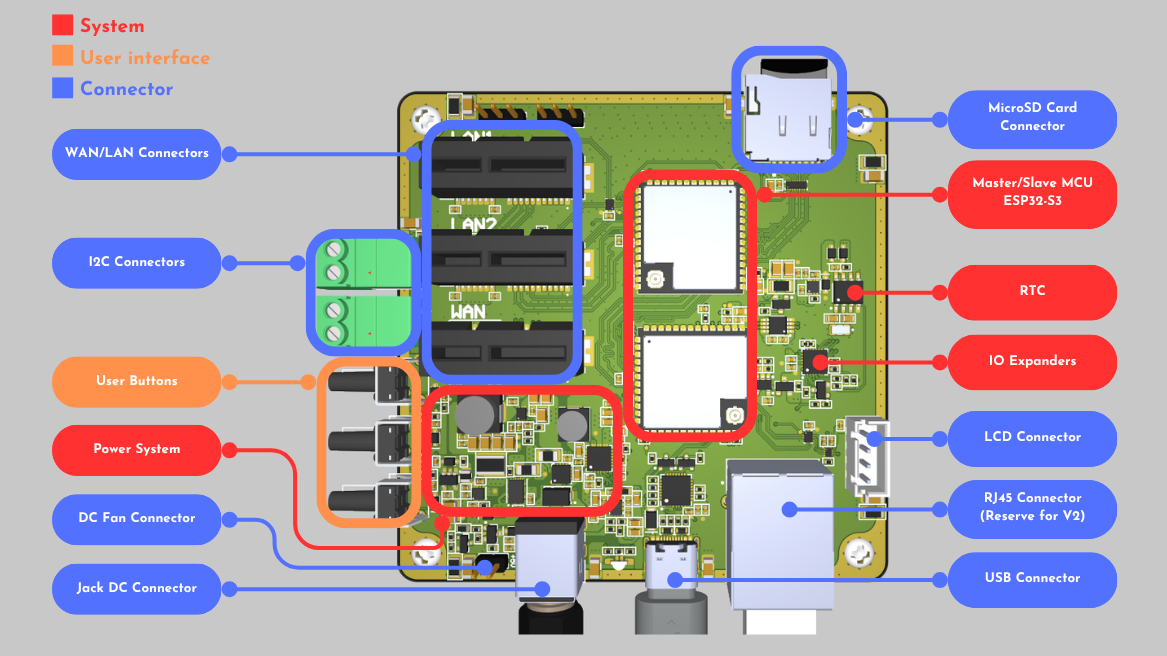
\includegraphics[width=0.9\textwidth]{figures/DATN/Assembly_Diagram_Top.png}
    \caption{Top Assembly Diagram }
\end{figure}
\begin{figure}[h]
    \centering
    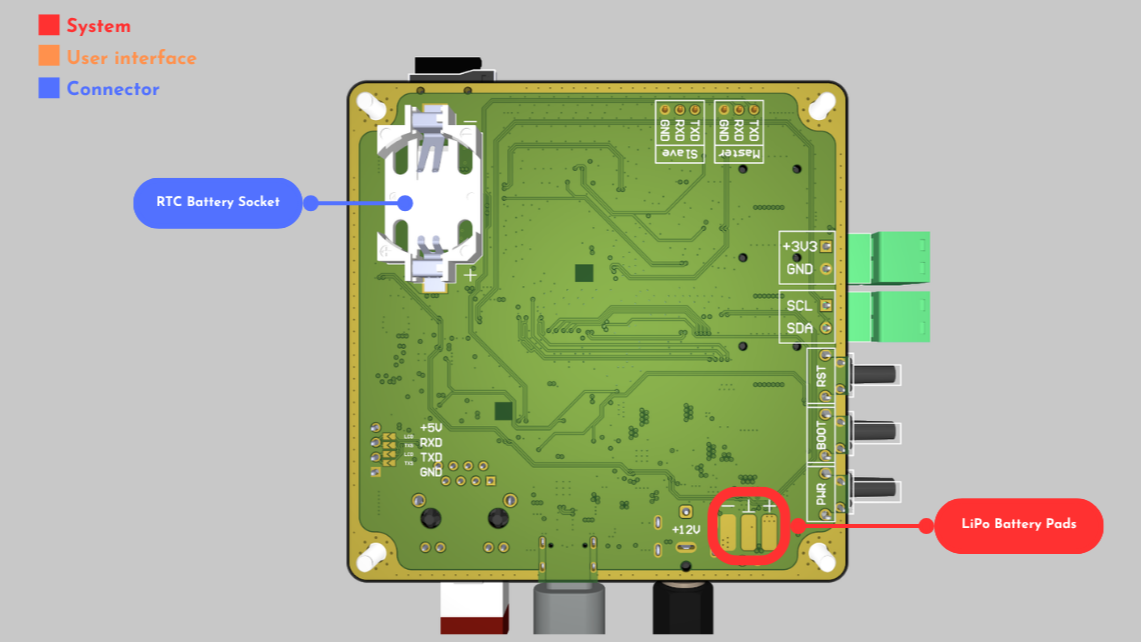
\includegraphics[width=0.9\textwidth]{figures/DATN/Assembly_Diagram_Bottom.png}
    \caption{Bottom Assembly Diagram }
\end{figure}
% \newpage
% \begin{figure}[h]
%     \centering
%     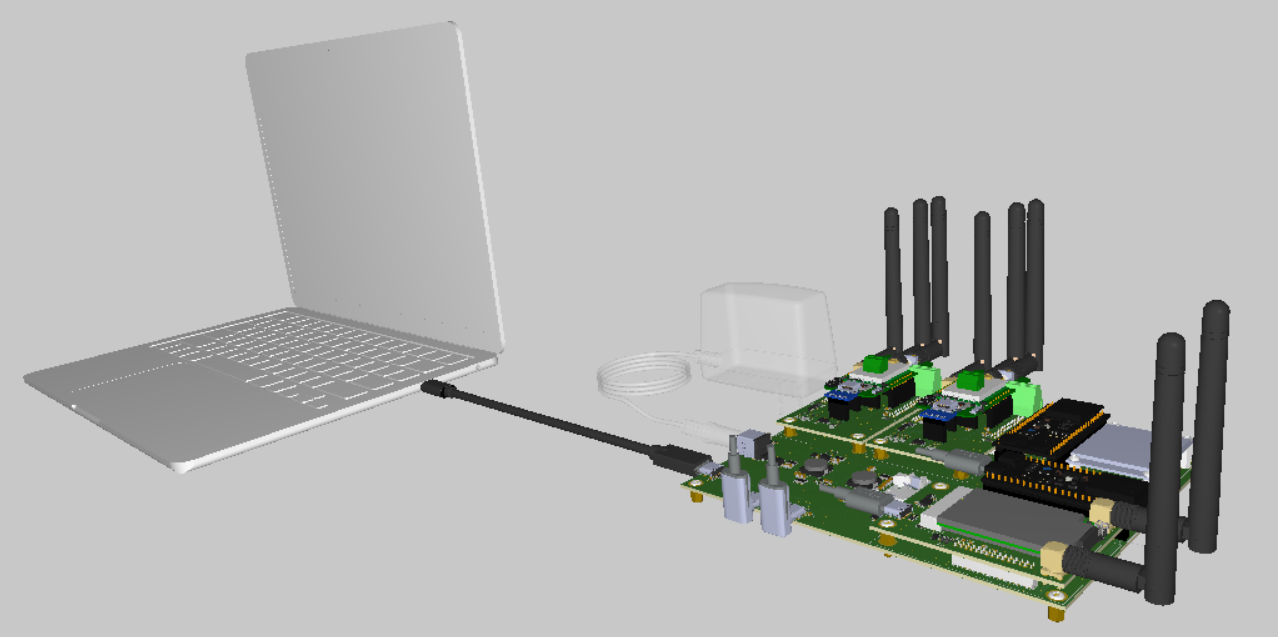
\includegraphics[width=0.8\textwidth]{figures/assembly_3d.png}
%     \caption{Mô hình 3D kết nối thiết bị.}
% \end{figure}

\begin{enumerate}
    \item \textbf{Bo mạch chủ (Baseboard):}
    Bo mạch chủ tích hợp hai vi điều khiển ESP32-S3 (Master và Slave) cùng hệ thống quản lý nguồn tập trung. Hệ thống nguồn cung cấp đồng thời các ray 12V, 5V, 3.3V và 1.8V để cấp nguồn cho các module.    
    
    \item \textbf{Cơ chế kết nối Module Adapter:}
    Việc lắp ráp các module chức năng được thông qua các chân cắm \textbf{WAN, LAN1, LAN2 Adapter Connection} đã được định nghĩa sẵn trên Baseboard:
    \begin{itemize}
        \item \textbf{Khe cắm WAN:} Thường lắp ráp các module kết nối mạng không dây như Wi-Fi/LTE/4G hoặc Ethernet.
        \item \textbf{Khe cắm LAN1/LAN2:} Dành cho các module giao tiếp công nghiệp hoặc mạng nội bộ như RS485, CAN Bus, LoRa hoặc Zigbee.
    \end{itemize}
    
    \item \textbf{Programmer USB-C:}
    Cổng USB-C sử dụng cho việc cấu hình IoT Gateway.
\end{enumerate}

\begin{figure}[h]
    \centering
    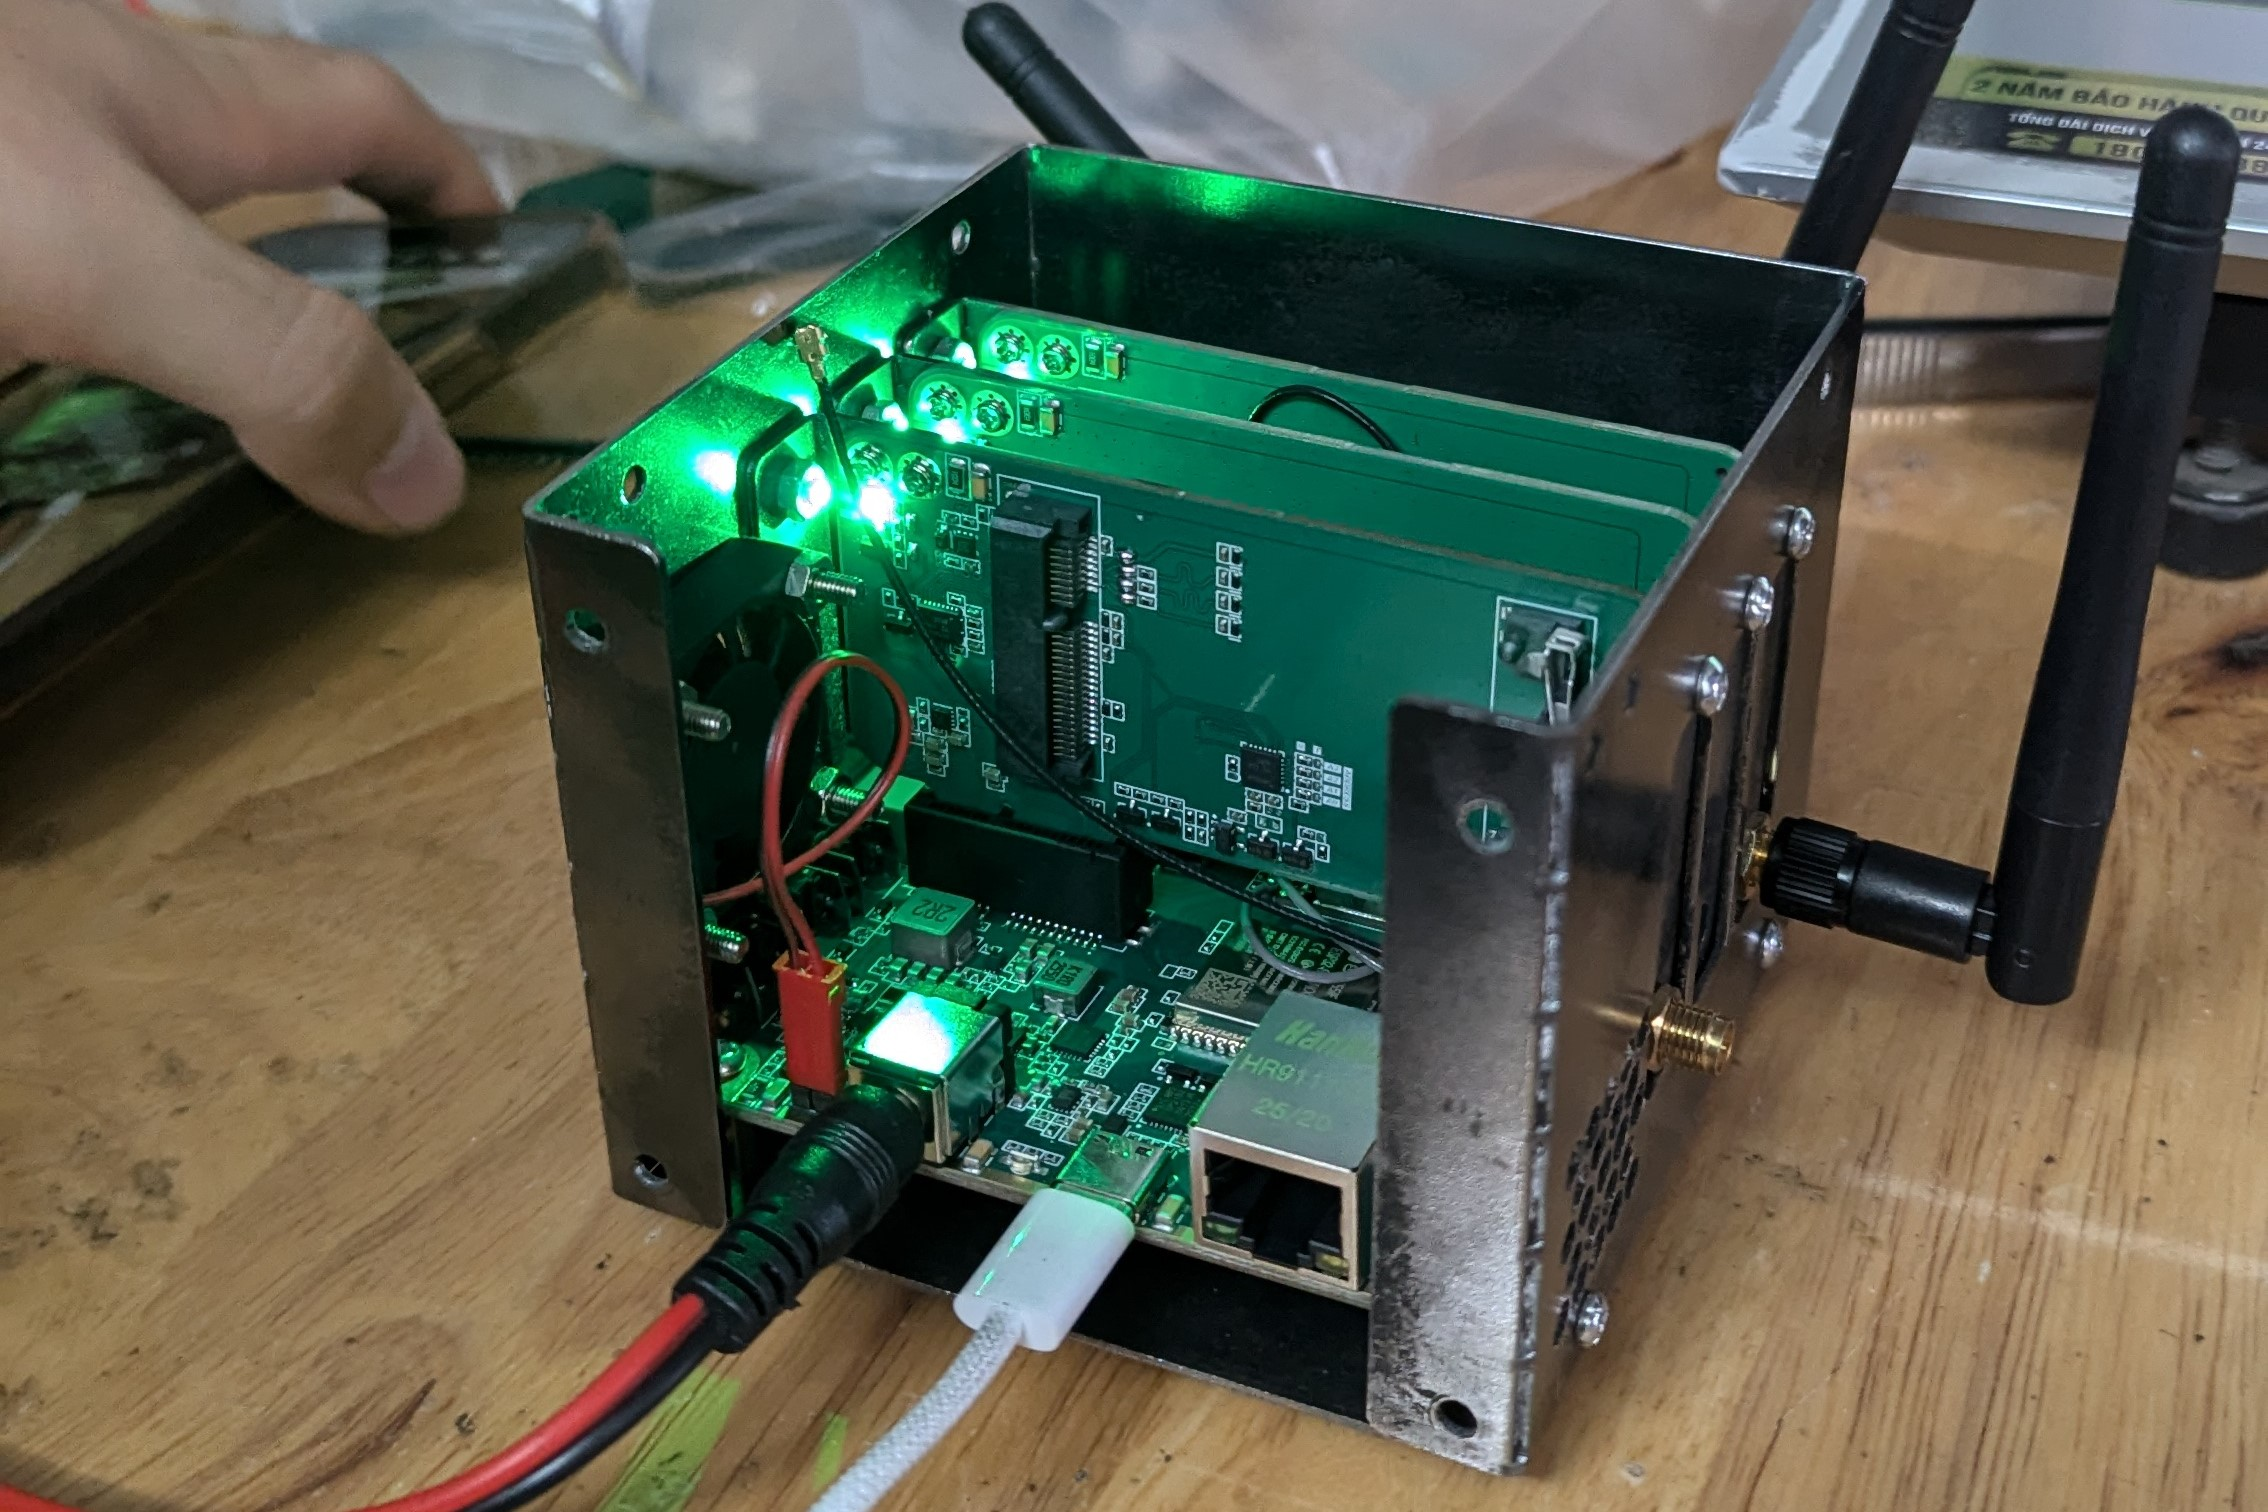
\includegraphics[width=0.7\textwidth]{figures/DATN/assembly_real.jpg}
    \caption{Hình ảnh sản phẩm thực tế.}
\end{figure}

% \newpage

\begin{figure}[H]
    \centering
    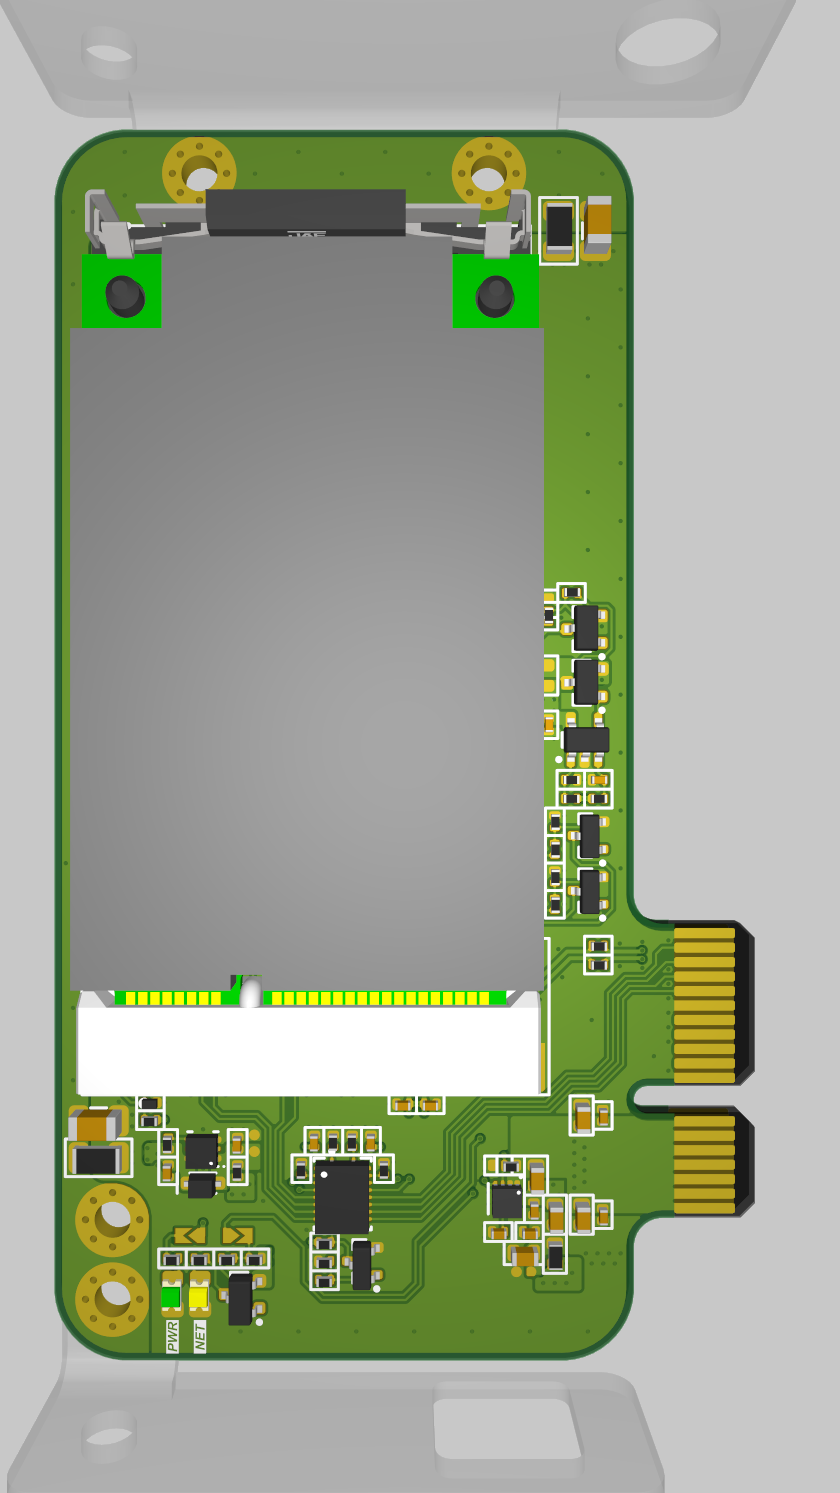
\includegraphics[width=0.25\textwidth]{figures/DATN/wan_adapter_lte.png}
    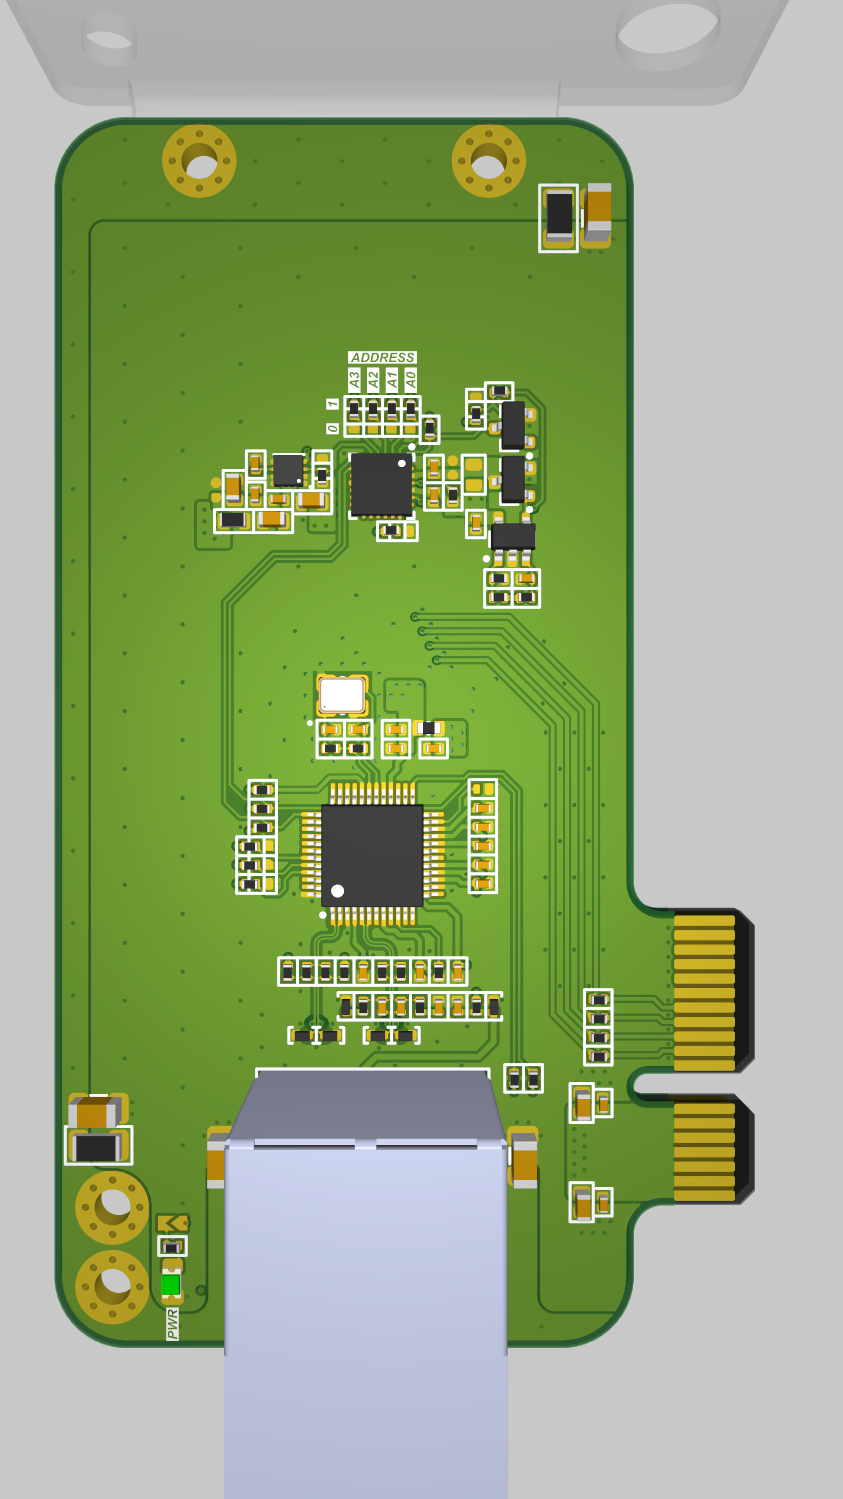
\includegraphics[width=0.25\textwidth]{figures/DATN/wan_adapter_ethernet.png}
    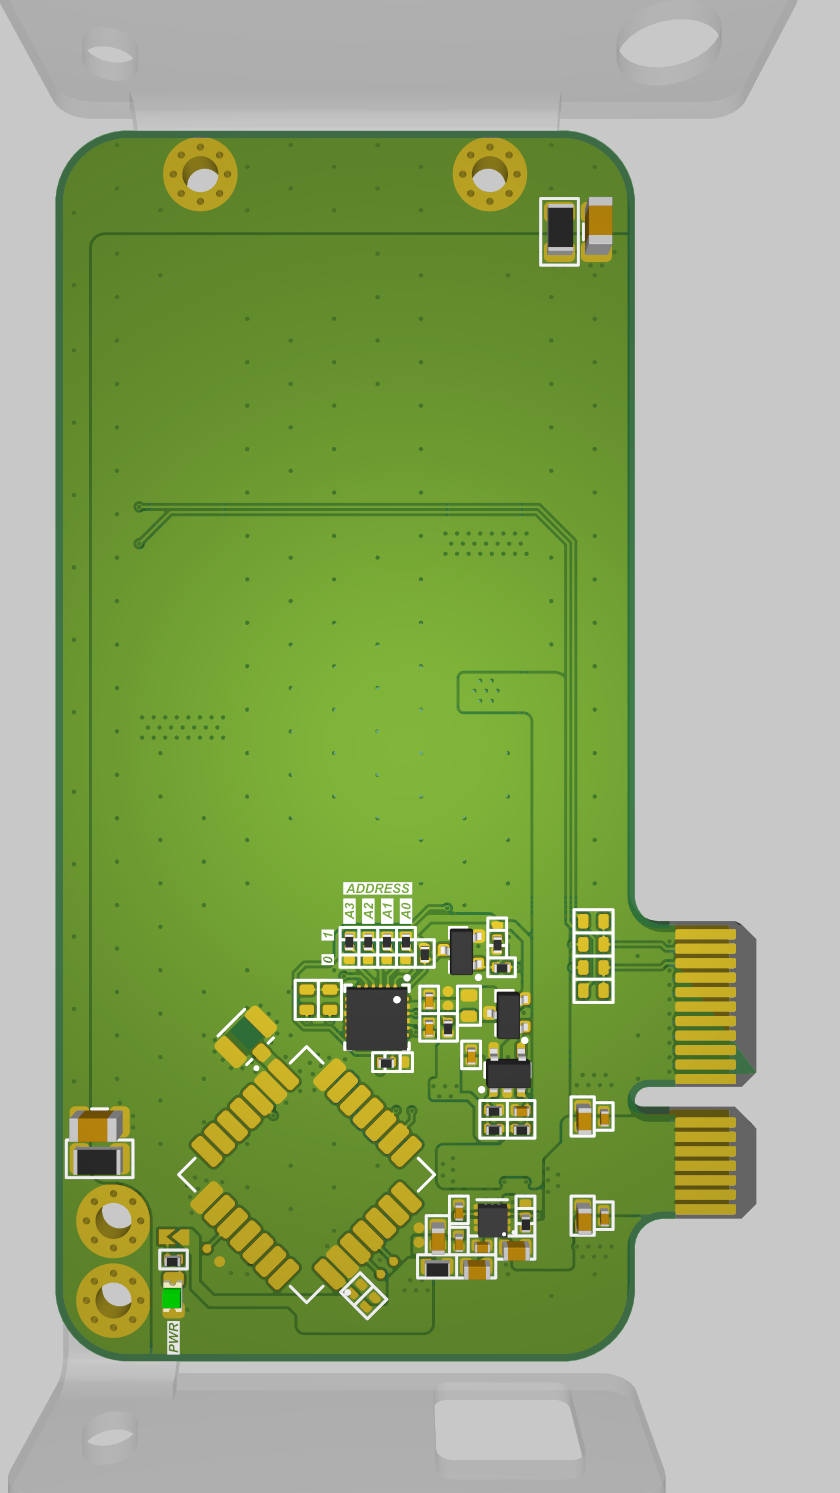
\includegraphics[width=0.25\textwidth]{figures/DATN/lan_adapter_lorawan.png}
    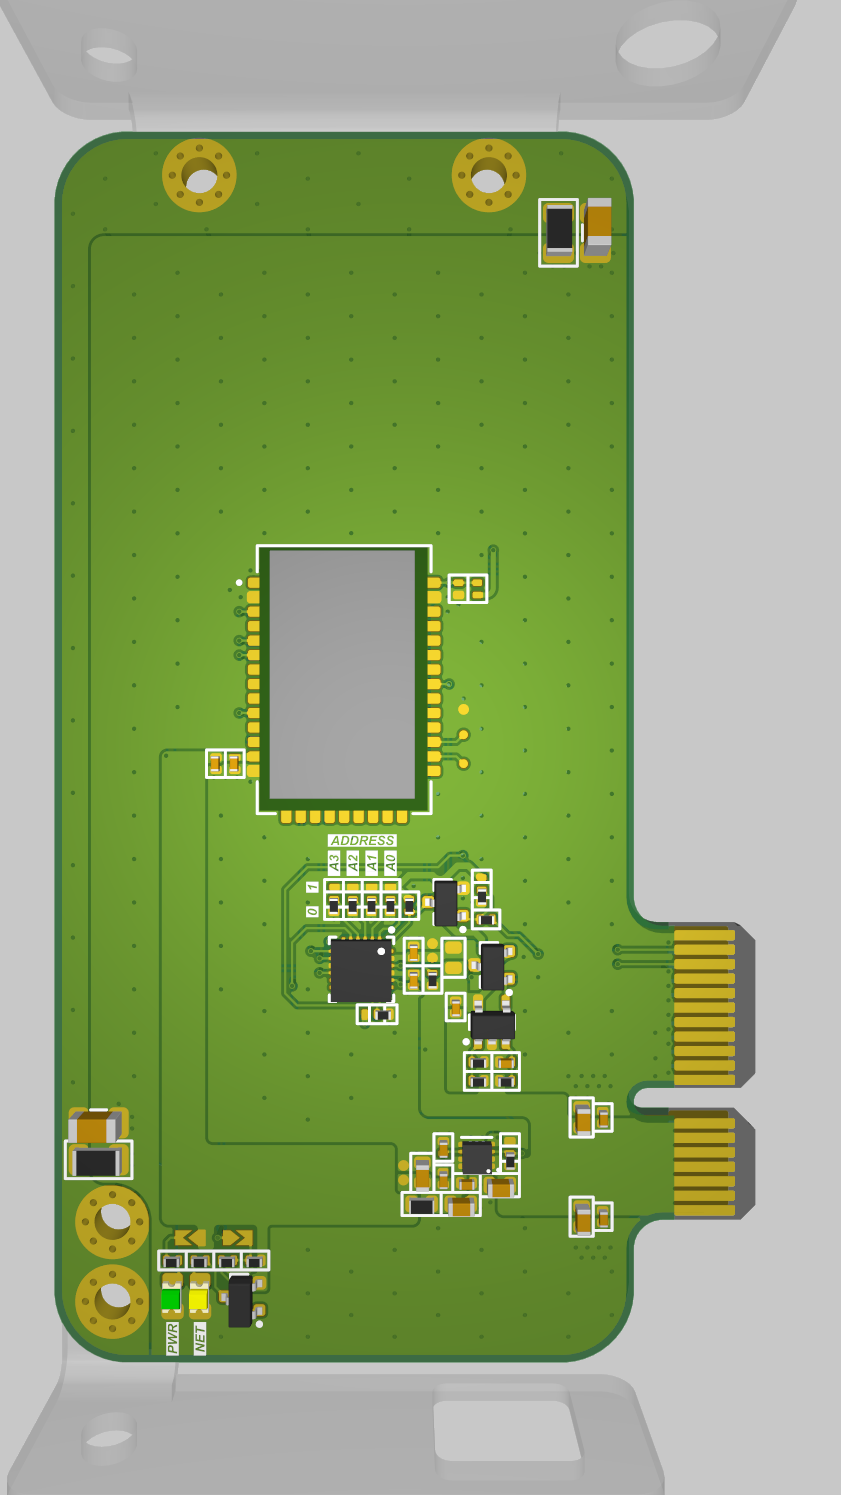
\includegraphics[width=0.25\textwidth]{figures/DATN/lan_adapter_zigbee.png}
    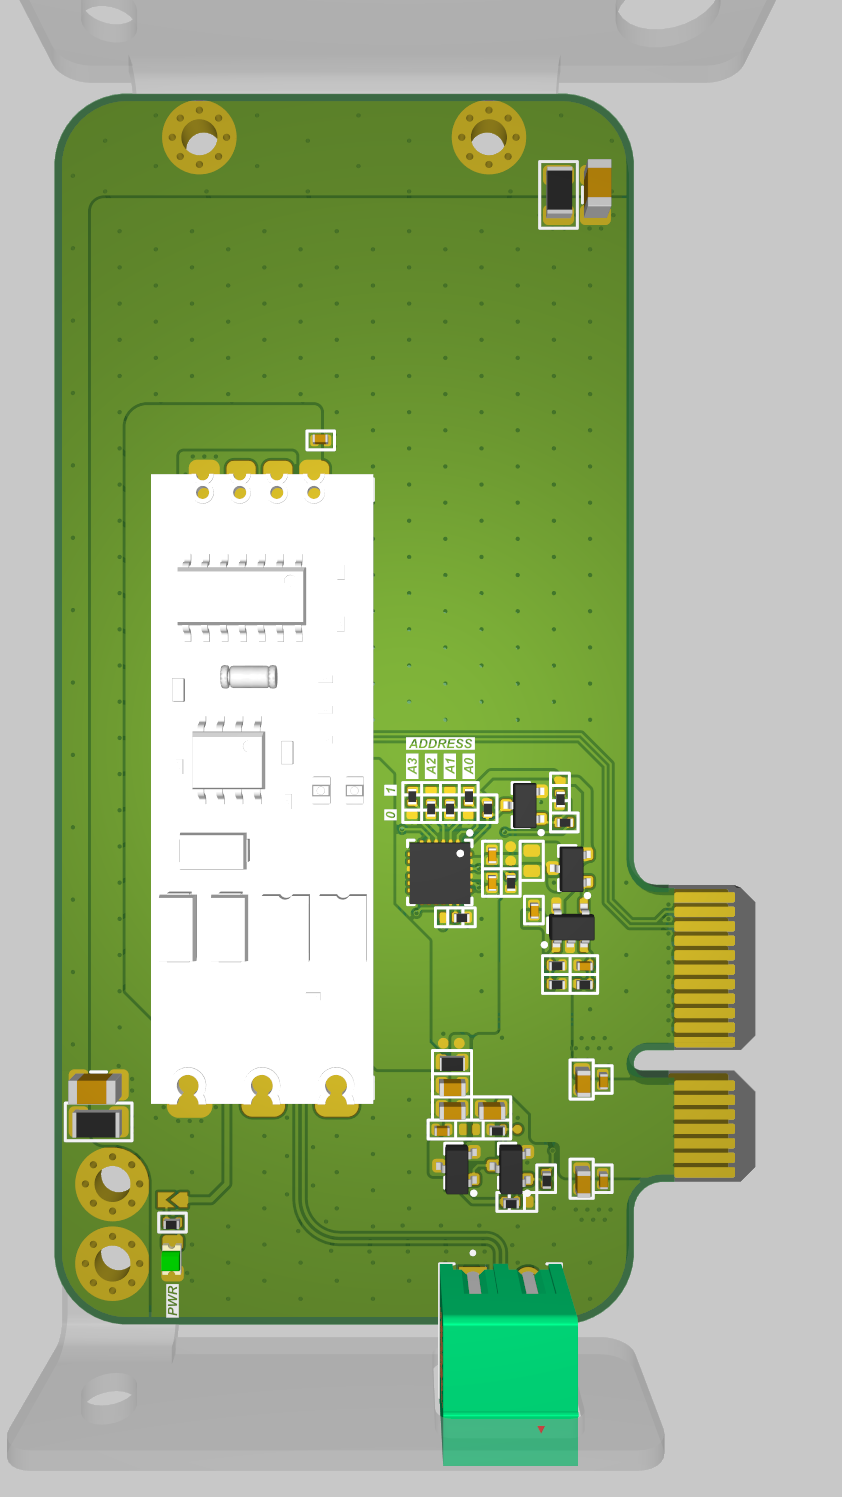
\includegraphics[width=0.25\textwidth]{figures/DATN/lan_adapter_rs485.png}
    \caption{Các Module Adapter đang hỗ trợ.}
\end{figure}
